\documentclass{article}

\usepackage{lmodern}
\usepackage[T1]{fontenc}
\usepackage{booktabs}
\usepackage{tabularx}
\usepackage{longtable}
\usepackage{array}
\usepackage{float}
\usepackage{pdflscape}
\usepackage{enumitem}
\usepackage{tikz}
\usetikzlibrary{arrows.meta, positioning, fit, backgrounds}
\usepackage[round]{natbib}
\usepackage{fullpage}
\usepackage{hyperref}

\hypersetup{
    colorlinks=true,       % false: boxed links; true: colored links
    linkcolor=red,          % color of internal links (change box color with linkbordercolor)
    citecolor=green,        % color of links to bibliography
    filecolor=magenta,      % color of file links
    urlcolor=cyan           % color of external links
}

\title{Hazard Analysis\\\progname}

\author{\authname}

\date{}

\input{../Comments.text}
\input{../Common.text}

% Ragged-right paragraph column for tables
\newcolumntype{L}[1]{>{\raggedright\arraybackslash}p{#1}}

% Hazards (H), safety and security requirements (SSR), losses (L),
% components (C) and critical assumptions (CA). Each \...def creates an anchor
% and each \...ref links to it.
\newcommand{\hazdef}[1]{\leavevmode\phantomsection\label{haz:#1}#1}
\newcommand{\hazref}[1]{\hyperref[haz:#1]{#1}}
\newcommand{\ssrdef}[1]{\phantomsection\label{ssr:#1}\textbf{SSR#1:}}
\newcommand{\ssrref}[1]{\hyperref[ssr:#1]{SSR#1}}
\newcounter{lossnum}
\newcommand{\lossdef}[1]{\refstepcounter{lossnum}\label{#1}\textbf{L\thelossnum:}}
\newcommand{\lossref}[1]{\hyperref[#1]{L\ref*{#1}}}
\newcounter{canum}
\newcommand{\cadef}[1]{\refstepcounter{canum}\label{#1}\textbf{CA\thecanum:}}
\newcommand{\caref}[1]{\hyperref[#1]{CA\ref*{#1}}}
\newcommand{\compref}[1]{\hyperref[comp:#1]{#1}}
\newcommand{\attr}[2]{\par\noindent\textit{#1:} #2}

% Links to the other project documents. Requirement identifiers such as FR9
% and NFR1 refer to the Software Requirements Specification, Revision 0.
\newcommand{\repourl}{https://github.com/team-hindsight/ophthamology-game}
\newcommand{\srsdoc}{\href{\repourl/blob/main/pdfs/SRS-IEEE/SRS.pdf}{Software Requirements Specification (SRS)}}
\newcommand{\srs}{\href{\repourl/blob/main/pdfs/SRS-IEEE/SRS.pdf}{SRS}}
\newcommand{\vnvplan}{\href{\repourl/blob/main/pdfs/VnVPlan/VnVPlan.pdf}{Verification and Validation (VnV) Plan}}
\newcommand{\dpdoc}{\href{\repourl/blob/main/pdfs/DevelopmentPlan/DevelopmentPlan.pdf}{Development Plan}}
\newcommand{\issue}[1]{\href{\repourl/issues/#1}{\##1}}

\setlength{\emergencystretch}{3em}
\setlist[itemize]{topsep=2pt, itemsep=2pt}

\begin{document}

\pagenumbering{roman}

\maketitle

~\newpage

\begin{table}[hp]
\caption{Revision History} \label{TblRevisionHistory}
\begin{tabularx}{\textwidth}{llX}
\toprule
\textbf{Date} & \textbf{Developer(s)} & \textbf{Change}\\
\midrule
2026-10-07 & Jake Finlay & First complete draft of Revision 0: all sections,
FMEA of eight components, 28 safety and security requirements, roadmap and
traceability.\\
\bottomrule
\end{tabularx}
\end{table}

~\newpage

\tableofcontents

\listoffigures

\listoftables

~\newpage

\pagenumbering{arabic}

\section{Introduction}
\label{sec_Intro}

This document is the hazard analysis for \progname{}, a mobile game that
prepares children aged three to seven for paediatric eye appointments. It
identifies the ways in which \progname{} could fail or behave so as to harm its
users or other stakeholders, and derives the safety and security requirements
that eliminate or reduce those hazards.

\subsection{Purpose}

The purpose of the analysis is to find hazards early, while they can still be
removed through the requirements rather than patched in the code. The safety
and security requirements of Section~\ref{sec_SSR} have been added to the
\srsdoc{}, so the hazard analysis directly shapes the design, implementation
and testing of the product. The analysis does not aim for zero risk, which is
not achievable, but for risk that is as low as reasonably practicable.

\subsection{Background}

Children are often anxious at eye appointments, and anxious children cooperate
less, which makes examinations longer and less complete. \progname{} walks a
child through each clinic procedure (eye drops, vision test, slit lamp
examination and others) with a friendly doctor character, lets the child
practise what the clinician will ask (such as keeping the eyes open), and
rewards each completed walkthrough with a sticker. A caregiver can choose the
procedures of the next visit and see what the child has practised. The product
runs offline on the family's phone or tablet and holds no personal
information. The full description of the product is in Sections~1 and 2 of the
\srs{}.

\progname{} controls no equipment and does not make clinical decisions, so it
cannot directly injure anyone in the way an insulin pump can. Its users,
however, are young children in a medical setting, and the product exists to
change how they feel about their care. Content that is wrong, frightening or
dishonest, activities that make a child feel they have failed, a privacy
failure, or a design that frustrates or over-engages the child can all cause
real harm. The analysis therefore uses a broad definition of harm, given
below.

\subsection{Definition of Hazard}
\label{sec_HazardDef}

Following \citet{Leveson2011}, a \emph{hazard} is a property or condition of
the system that, together with a condition in its environment, has the
potential to cause a loss. A \emph{loss} is harm or damage to a stakeholder.
As recommended for capstone projects, ``harm'' is not limited to physical
injury: it includes psychological harm to children, privacy and security
breaches, care decisions made on wrong information, harm to well-being, loss
of the child's preparation, and loss of the product's ability to serve its
users. The losses considered are listed in Table~\ref{tab:Losses}.

\subsection{Document Roadmap}

Section~\ref{sec_Scope} states the scope of the analysis and the losses it
considers. Section~\ref{sec_Boundary} defines the system boundary and divides
\progname{} into the components that the analysis examines.
Section~\ref{sec_Assumptions} lists the critical assumptions.
Section~\ref{sec_FMEA} explains the Failure Mode and Effect Analysis (FMEA)
method and presents the FMEA tables, one per component.
Section~\ref{sec_SSR} lists the safety and security requirements derived from
the FMEA, and Section~\ref{sec_Roadmap} states when each will be implemented.
Appendix~\ref{sec_Matrix} gives the full traceability between hazards and
requirements, followed by the generative AI disclosure and the reflection.

\subsection{Template Changes}

The sections of the course template are kept in its order. The following were
added: a list of figures and tables; the table of losses
(Section~\ref{sec_Scope}); the definitions of severity and of mitigation
strategy categories (Section~\ref{sec_FMEAMethod}); one FMEA table per
component instead of a single table; and the traceability matrix of
Appendix~\ref{sec_Matrix}.

\section{Scope and Purpose of Hazard Analysis}
\label{sec_Scope}

\paragraph{In scope.} The analysis covers \progname{} as specified in the
\srs{}, Revision 0: every functional area of the app, its Procedure Content,
its stored data, its interaction with the device's operating system (OS), its
distribution through the app stores, and the process by which its content is
produced and approved before release. Hazards that arise from how people are
likely to use, or misuse, the product (for example, treating it as medical
advice) are included.

\paragraph{Out of scope.} The clinical procedures themselves and the conduct
of the clinic; the device hardware and OS, except for how \progname{} responds
to their failures; the clinic's record systems; and the stretch goals
(augmented reality and personalization), which will need their own analysis if
adopted (SRS likely changes LC8 and LC9). The usability study with children is
outside the product but is included as one process hazard
(\hazref{H8-2}), because its harms fall on the same users.

\paragraph{Losses.} Table~\ref{tab:Losses} lists the losses that the hazards
could lead to. Every hazard in Section~\ref{sec_FMEA} leads to at least one of
them.

\begin{table}[H]
\centering
\caption{Losses considered by the hazard analysis}
\label{tab:Losses}
\begin{tabular}{lL{0.75\textwidth}}
\toprule
\textbf{ID} & \textbf{Loss}\\
\midrule
\lossdef{L_Physical} & Physical harm to a child, such as a photosensitive
seizure or hearing discomfort.\\
\lossdef{L_Psych} & Psychological harm to a child: increased fear or anxiety
about the appointment, shame, or loss of trust in caregivers or clinicians.\\
\lossdef{L_Care} & Harm to the child's care: a less complete or longer
examination, or a care decision based on wrong information.\\
\lossdef{L_Privacy} & Disclosure or misuse of personal information about a
child or family.\\
\lossdef{L_Wellbeing} & Harm to well-being, such as excessive or compulsive
use, or harm to self-image.\\
\lossdef{L_Preparation} & Loss of the child's preparation: the child cannot use
\progname{}, cannot finish a walkthrough, or loses earned progress.\\
\lossdef{L_Trust} & Loss of trust in the product by families and clinicians,
or its removal from the app stores.\\
\bottomrule
\end{tabular}
\end{table}

\section{System Boundaries and Components}
\label{sec_Boundary}

The system analysed is \progname{} running on a family's phone or tablet,
together with the release process that puts content and builds into it.
Figure~\ref{fig:Boundary} shows the boundary and the components, and
Table~\ref{tab:Components} describes each component. The components are
functional, not a design: they follow the functional areas of the \srs{}
(Section~2.3) and will be refined in the design documents.

\begin{figure}[H]
\centering
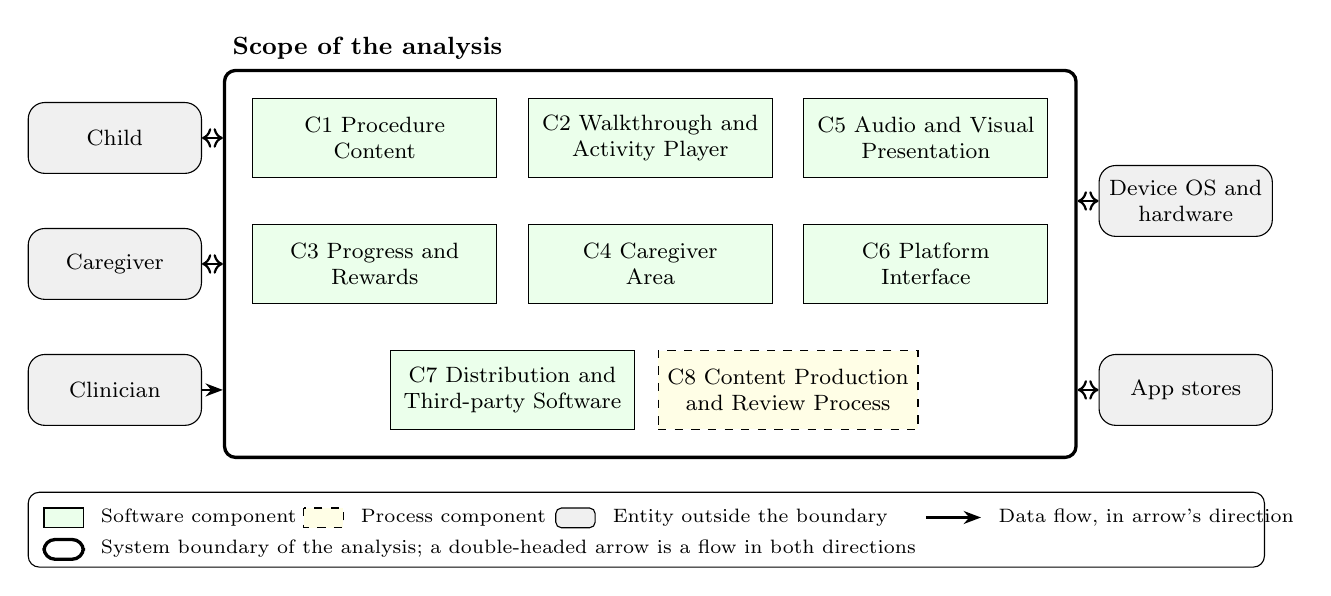
\begin{tikzpicture}[
  font=\small,
  comp/.style={draw, fill=green!8, align=center, minimum width=3.1cm,
    minimum height=1.0cm, font=\footnotesize},
  proc/.style={draw, dashed, fill=yellow!10, align=center, minimum width=3.1cm,
    minimum height=1.0cm, font=\footnotesize},
  ext/.style={draw, rounded corners=6pt, fill=gray!12, align=center,
    minimum width=2.2cm, minimum height=0.9cm, font=\footnotesize},
  flow/.style={-{Stealth[length=2.2mm]}, thick},
]
\node[comp] (c1) at (0, 2.4) {C1 Procedure\\Content};
\node[comp] (c2) at (3.5, 2.4) {C2 Walkthrough and\\Activity Player};
\node[comp] (c5) at (7.0, 2.4) {C5 Audio and Visual\\Presentation};
\node[comp] (c3) at (0, 0.8) {C3 Progress and\\Rewards};
\node[comp] (c4) at (3.5, 0.8) {C4 Caregiver\\Area};
\node[comp] (c6) at (7.0, 0.8) {C6 Platform\\Interface};
\node[comp] (c7) at (1.75, -0.8) {C7 Distribution and\\Third-party Software};
\node[proc] (c8) at (5.25, -0.8) {C8 Content Production\\and Review Process};
\begin{scope}[on background layer]
\node[draw, very thick, rounded corners, inner sep=0.35cm,
  fit=(c1) (c2) (c5) (c3) (c4) (c6) (c7) (c8)] (sys) {};
\end{scope}
\node[anchor=south west, font=\small\bfseries] at (sys.north west)
  {Scope of the analysis};

\node[ext] (child) at (-3.3, 2.4) {Child};
\node[ext] (care) at (-3.3, 0.8) {Caregiver};
\node[ext] (clin) at (-3.3, -0.8) {Clinician};
\node[ext] (os) at (10.3, 1.6) {Device OS and\\hardware};
\node[ext] (store) at (10.3, -0.8) {App stores};

\draw[flow, <->] (child) -- (sys.west |- child);
\draw[flow, <->] (care) -- (sys.west |- care);
\draw[flow] (clin) -- (sys.west |- clin);
\draw[flow, <->] (os) -- (sys.east |- os);
\draw[flow, <->] (store) -- (sys.east |- store);

\begin{scope}[shift={(-4.3, -2.4)}, font=\scriptsize]
  \draw[rounded corners] (-0.1, 0.3) rectangle (15.6, -0.65);
  \draw[fill=green!8] (0.1, 0.1) rectangle (0.6, -0.15);
  \node[anchor=west] at (0.7, -0.02) {Software component};
  \draw[dashed, fill=yellow!10] (3.4, 0.1) rectangle (3.9, -0.15);
  \node[anchor=west] at (4.0, -0.02) {Process component};
  \draw[rounded corners=2pt, fill=gray!12] (6.6, 0.1) rectangle (7.1, -0.15);
  \node[anchor=west] at (7.2, -0.02) {Entity outside the boundary};
  \draw[flow] (11.3, -0.02) -- (12.0, -0.02);
  \node[anchor=west] at (12.1, -0.02) {Data flow, in arrow's direction};
  \draw[very thick, rounded corners] (0.1, -0.3) rectangle (0.6, -0.55);
  \node[anchor=west] at (0.7, -0.42) {System boundary of the analysis; a
    double-headed arrow is a flow in both directions};
\end{scope}
\end{tikzpicture}
\caption{System boundary and components of \progname{} for the hazard
analysis}
\label{fig:Boundary}
\end{figure}

\begin{longtable}{lL{0.22\textwidth}L{0.62\textwidth}}
\caption{Components analysed} \label{tab:Components}\\
\toprule
\textbf{ID} & \textbf{Component} & \textbf{Responsibilities and SRS
reference}\\
\midrule
\endfirsthead
\toprule
\textbf{ID} & \textbf{Component} & \textbf{Responsibilities and SRS
reference}\\
\midrule
\endhead
\phantomsection\label{comp:C1}C1 & Procedure Content & The narration,
captions, illustrations, sensation warnings, Knowledge Check answers and
caregiver guides for each procedure (SRS Section~7).\\
\phantomsection\label{comp:C2}C2 & Walkthrough and Activity Player & Presents
the steps of a walkthrough and applies the rules of the activities (SRS
Sections~6.2, 6.3 and 6.9).\\
\phantomsection\label{comp:C3}C3 & Progress and Rewards & Records completions,
dates and stickers on the device (SRS Section~6.4).\\
\phantomsection\label{comp:C4}C4 & Caregiver Area & Notice, Caregiver Check,
procedure guide, settings, Visit Plan and Visit Code, Practice Summary and reset
(SRS Sections~6.5 and 6.6).\\
\phantomsection\label{comp:C5}C5 & Audio and Visual Presentation & Narration,
sound effects, animations, captions and visual cues (SRS Section~6.7).\\
\phantomsection\label{comp:C6}C6 & Platform Interface & Touch input,
life-cycle events, storage and performance on the device (SRS
Section~6.8).\\
\phantomsection\label{comp:C7}C7 & Distribution and Third-party Software & The
release build, its signing, its store listing, and any third-party libraries
and assets it includes.\\
\phantomsection\label{comp:C8}C8 & Content Production and Review Process & How
content is written, reviewed by clinicians and child-life experts, and
released; also the usability study with children.\\
\bottomrule
\end{longtable}

\noindent Inputs to the system are the child's touches, the caregiver's entries
(including Visit Codes provided by the clinic), OS life-cycle events, stored
data, and released content and builds. Outputs are what the child and
caregiver see and hear, and the data stored on the device. The complete list
is in Table~4 of the \srs{}.

\section{Critical Assumptions}
\label{sec_Assumptions}

The assumptions below limit the hazards that must be mitigated. They were kept
to a minimum: in particular, the analysis does \emph{not} assume that the
software is free of defects, that stored data is always valid, that the device
never interrupts the app, or that caregivers read instructions.

\begin{itemize}[leftmargin=1.4cm, labelwidth=1.2cm, align=left]
\item[\cadef{CA_NotMalicious}] Users do not deliberately tamper with the app's
  stored data or installed package. Accidental corruption is still analysed
  (\hazref{H3-1}), and malicious third parties are considered in
  \hazref{H7-3}.
\item[\cadef{CA_Supervision}] A caregiver is responsible for the child's use of
  the device and installs the app. The Caregiver Check is a barrier against
  young children, not against a determined older child.
\item[\cadef{CA_OS}] The device OS isolates the app's private storage from
  other apps and enforces app signing. \progname{} relies on this instead of
  encrypting its non-personal data.
\item[\cadef{CA_ClinicalReviewers}] Clinicians and a child-life specialist (or
  child development expert) are available to review content. If they are not,
  content is not released (\ssrref{1}, \ssrref{3}); this assumption affects the
  amount of content, not its safety.
\item[\cadef{CA_NotSaMD}] \progname{} is used for preparation and education
  only, as stated in its notice. The hazard that it is used otherwise is still
  analysed (\hazref{H1-4}).
\end{itemize}

\section{Failure Mode and Effect Analysis}
\label{sec_FMEA}

\subsection{Method}
\label{sec_FMEAMethod}

The analysis uses Failure Mode and Effects Analysis (FMEA), as described in
the course lectures and in IEC 60812 \citep{IEC60812_2018}. FMEA was chosen
because it works bottom-up from the components of
Section~\ref{sec_Boundary}, which are already known from the SRS, and because
most hazards of \progname{} arise from single failures (one piece of wrong
content, one unhandled event) rather than from complex control interactions,
for which System-Theoretic Process Analysis would be more suited. The
medical-device standards ISO 14971 \citep{ISO14971_2019} and IEC 62304
\citep{IEC62304_2015} were consulted for the kinds of hazards to consider,
such as incorrect information and use error, although \progname{} is not a
medical device.

For each component, the team asked how each of its functions could fail. Each
row of the FMEA tables records:

\begin{itemize}
\item \textbf{Design function:} what the component must do.
\item \textbf{Failure mode:} how the failure would be observed.
\item \textbf{Effects of failure:} the consequence for the child, the caregiver
  or the clinician, and the losses of Table~\ref{tab:Losses} it leads to.
\item \textbf{Causes of failure:} the reasons the failure could occur, labelled
  a, b, c\ldots
\item \textbf{Detection:} how the failure would be found, before release or
  while the app runs.
\item \textbf{Severity:} the worst credible effect, rated with
  Table~\ref{tab:Severity}.
\item \textbf{Recommended actions:} what will eliminate or mitigate the hazard,
  labelled to match the causes and tagged with a strategy from
  Table~\ref{tab:Strategy}. SRS requirements that already mitigate the hazard
  are cited by their SRS identifiers (FR or NFR).
\item \textbf{SSR:} the safety and security requirements of
  Section~\ref{sec_SSR} that the actions lead to.
\item \textbf{Ref:} the hazard identifier, H$c$-$n$ for the $n$-th hazard of
  component C$c$.
\end{itemize}

\noindent The analysis rates severity but deliberately does not compute a Risk
Priority Number from estimated probabilities. As the course lecture notes,
there is seldom a sound basis for such estimates, and accidents have resulted
from hazards judged ``unlikely''. Every identified hazard therefore receives a
recommended action, whatever its estimated likelihood, and severity is used
only to order the work in the roadmap (Section~\ref{sec_Roadmap}).

\begin{table}[H]
\centering
\caption{Severity classification}
\label{tab:Severity}
\begin{tabular}{lL{0.75\textwidth}}
\toprule
\textbf{Severity} & \textbf{Worst credible effect}\\
\midrule
S4 Catastrophic & Physical injury to a child, a care decision that could
cause physical harm, or disclosure of a child's personal information.\\
S3 Critical & Significant distress or loss of trust around the appointment, or
a failure of preparation that may compromise the examination.\\
S2 Moderate & Frustration or upset that the child recovers from during use,
or reduced preparation.\\
S1 Minor & Inconvenience with no effect on the child's preparation.\\
\bottomrule
\end{tabular}
\end{table}

\begin{table}[H]
\centering
\caption{Categories of recommended action}
\label{tab:Strategy}
\begin{tabular}{lL{0.72\textwidth}}
\toprule
\textbf{Category} & \textbf{Meaning}\\
\midrule
{[E]} Eliminate & Remove the hazard, for example by not providing the feature
that creates it.\\
{[M]} Mitigate & Reduce the likelihood of the failure or the severity of its
effect at run time.\\
{[D]} Document & Warn or inform users, or record a procedure that people must
follow.\\
{[V]} Verify & Add a review or test that detects the failure before
release.\\
\bottomrule
\end{tabular}
\end{table}

\subsection{FMEA Tables}
\label{sec_FMEATables}

Tables~\ref{tab:FMEA-C1} to \ref{tab:FMEA-C8} give the FMEA for components C1
to C8. They are printed in landscape orientation.

% Column widths for every FMEA table (landscape \textwidth is the page height)
\newcolumntype{F}{L{2.0cm}L{2.5cm}L{2.8cm}L{3.2cm}L{2.2cm}L{0.8cm}%
L{4.8cm}L{1.1cm}l}
\newcommand{\fmeahead}{\toprule
\textbf{Design function} & \textbf{Failure mode} & \textbf{Effects of failure}
& \textbf{Causes of failure} & \textbf{Detection} & \textbf{Sev.} &
\textbf{Recommended actions} & \textbf{SSR} & \textbf{Ref}\\
\midrule}

\begin{landscape}
\footnotesize
\setlength{\tabcolsep}{3pt}

\begin{longtable}{F}
\caption{FMEA for component C1, Procedure Content} \label{tab:FMEA-C1}\\
\fmeahead
\endfirsthead
\fmeahead
\endhead
Depict each procedure accurately & Procedure shown inaccurately (wrong steps,
order, equipment or timing) & Child's expectations do not match the clinic:
surprise, anxiety, reduced cooperation; clinicians stop recommending the app
(\lossref{L_Psych}, \lossref{L_Care}, \lossref{L_Trust}) & a.~No team member
has clinical training. b.~Procedures differ between clinics. c.~Clinical
practice changes after release. & Clinician review; observation in
usability sessions & S3 & a.~[V] Clinician approval of every content version
before release. b.~[D] Content says the child's doctor may do things a little
differently. c.~[V] Content re-reviewed when practice changes; the approved
version is recorded. & \ssrref{1} & \hazdef{H1-1}\\
\addlinespace
Prepare the child honestly for sensations & Unpleasant sensation omitted or
played down (``it won't hurt'') & Child is surprised by burning drops or a
bright light: distress and loss of trust in caregivers, clinicians and the app
(\lossref{L_Psych}, \lossref{L_Trust}) & a.~Writers try to reassure. b.~The
warning is skipped by fast tapping. & Child-life review; inspection & S3 &
a.~[M] Every step with a sensation tag presents a warning before its activity.
[V] Review forbids promises of no discomfort. b.~[E] The warning cannot be
skipped, and touches made before a step is shown are ignored. & \ssrref{2},
\ssrref{3}, \ssrref{28} & \hazdef{H1-2}\\
\addlinespace
Present the procedure in a calming way & Frightening content (needles, blood,
crying, looming equipment, sudden noises) & Increased fear of the appointment
(\lossref{L_Psych}) & a.~Realistic depiction chosen for accuracy. b.~Stock
assets used without review. & Child-life review & S3 & a, b.~[V] Child-life
review of all images, sounds and language, with an explicit list of excluded
content. & \ssrref{3} & \hazdef{H1-3}\\
\addlinespace
Stay a preparation aid & Content taken as medical advice (for example, how to
give drops at home, or that a symptom is normal) & Caregiver makes a care
decision based on the app (\lossref{L_Care}, \lossref{L_Physical}) & a.~The
doctor character sounds authoritative. b.~Caregiver guides explain
procedures. & None at run time; content review & S4 & a.~[D] Not-medical-advice
notice acknowledged at first launch and shown with every guide (SRS FR28,
FR29). b.~[E] No diagnostic, treatment or medication content (SRS NFR41). &
\ssrref{4} & \hazdef{H1-4}\\
\addlinespace
Represent all children & Characters and families stereotyped or not diverse
& Child feels excluded; harm to self-image, for example for a child with a
patch or glasses (\lossref{L_Wellbeing}, \lossref{L_Psych}) & a.~Limited
diversity of free assets. b.~Assumptions about family structure. & Review &
S2 & a.~[V] Representation criteria checked in review. b.~[M] Caregiver text
uses ``grown-up'' and ``caregiver''. & \ssrref{5} & \hazdef{H1-5}\\
\addlinespace
Prepare for the child's own visit & Child practises procedures that are not
in the visit and misses one that is & Child is surprised by an unprepared
procedure (\lossref{L_Psych}, \lossref{L_Preparation}) & a.~Caregiver does not
know which procedures are planned. b.~Too many procedures to do them all. &
None at run time & S2 & a.~[M] Visit Plan set by the caregiver or a clinic
code, shown first in the library. [D] Caregiver guide describes every
procedure. b.~[M] Visit Plan procedures listed first. & \ssrref{6} &
\hazdef{H1-6}\\
\addlinespace
Teach the right behaviour & Wrong behaviour rewarded (for example, a Knowledge
Check marks ``squeeze your eyes shut'' as correct) & Child does the wrong thing
at the clinic, so drops or tests must be repeated (\lossref{L_Care}) &
a.~Content error. b.~Wrong correct-answer index in the data. & Clinician
review; automatic content validation & S3 & a.~[V] Clinician approval covers
the answers. b.~[V] Automatic validation of the content constraints (SRS
NFR11). & \ssrref{1}, \ssrref{7} & \hazdef{H1-7}\\
\bottomrule
\end{longtable}

\begin{longtable}{F}
\caption{FMEA for component C2, Walkthrough and Activity Player}
\label{tab:FMEA-C2}\\
\fmeahead
\endfirsthead
\fmeahead
\endhead
Let the child finish every activity & Activity cannot be completed (no correct
answer, target unreachable or off-screen, player stuck) & Child is stuck:
frustration and a sense of failure before the appointment; walkthrough
abandoned (\lossref{L_Psych}, \lossref{L_Preparation}) & a.~Invalid content.
b.~Defect in the activity rules. c.~Target outside the visible area on an
unusual screen. & Automatic validation; tests of the formal no-dead-end
property; screen-size tests & S3 & a.~[V] Automatic content validation (SRS
NFR11). b.~[E] Activities can only end in success, with assistance after
repeated attempts; [V] property P1 of SRS Section~6.9 tested. c.~[V] Layout
tested on all aspect ratios (SRS NFR15). [M] Caregiver skip as a last
resort. & \ssrref{7} & \hazdef{H2-1}\\
\addlinespace
Respond kindly to mistakes & Punitive feedback (failure sound, red cross,
``wrong'') & Shame and anxiety (\lossref{L_Psych}) & a.~Common game
conventions copied by default. & Inspection; child-life review & S2 & a.~[E]
Feedback to mistakes is only encouraging; failure sounds, crosses, red and
negative words are excluded. & \ssrref{8} & \hazdef{H2-2}\\
\addlinespace
Suit the youngest children & Activity too hard for a three-year-old (hold too
long, question too hard) & Repeated unsuccessful attempts; frustration
(\lossref{L_Psych}) & a.~Durations chosen for older children. b.~Questions
beyond the child's understanding. & Usability sessions & S2 & a.~[M] Required
hold time shortened after repeated interruptions. b.~[M] Correct answer
highlighted after repeated wrong answers. [V] Constants tuned in usability
testing. & \ssrref{9}, \ssrref{7} & \hazdef{H2-3}\\
\addlinespace
Register the child's touches & Touches missed or misattributed & Child thinks
they did something wrong; frustration (\lossref{L_Psych}) & a.~Small targets.
b.~Slow response. c.~Several fingers or the palm on the screen. & Usability
sessions; performance tests & S2 & a.~[M] Minimum target size and spacing.
b.~[M] Response time limit. c.~[M] Multi-touch rules for holds and taps. &
\ssrref{10}, \ssrref{28} & \hazdef{H2-4}\\
\addlinespace
Present every step & Rapid tapping skips steps & Child misses information,
including sensation warnings (\lossref{L_Psych}) & a.~Taps queued during
transitions are applied to the next step. & Tests with random rapid taps &
S2 & a.~[E] A touch completes at most one step, and touches that began before a
step was shown are ignored. & \ssrref{28}, \ssrref{2} & \hazdef{H2-5}\\
\bottomrule
\end{longtable}

\begin{longtable}{F}
\caption{FMEA for component C3, Progress and Rewards} \label{tab:FMEA-C3}\\
\fmeahead
\endfirsthead
\fmeahead
\endhead
Keep the child's progress & Progress lost or corrupted, or the app fails at
launch because of it & Stickers disappear and the child is upset; in the worst
case the app cannot be used before the appointment (\lossref{L_Psych},
\lossref{L_Preparation}) & a.~App terminated while saving. b.~Storage full.
c.~Stored data corrupted. d.~An update changes the data format. & Validity
check of stored data at launch (SRS Section~6.9.5); fault-injection tests & S3
& a.~[M] Progress is saved so that the last valid state survives termination.
b.~[M] Save failures are retried without disturbing the child. c.~[M] Invalid
data is detected and the last valid state, or the initial state, is restored
without failing. d.~[V] Progress retained across updates is tested. &
\ssrref{11} & \hazdef{H3-1}\\
\addlinespace
Award stickers correctly & Sticker not awarded, or awarded twice & Confusion
and disappointment (\lossref{L_Psych}) & a.~Defect in the award logic. &
Tests of the progress invariant (SRS property P3) & S1 & a.~[V] Award rule and
invariant specified formally and tested. & \ssrref{11} & \hazdef{H3-2}\\
\addlinespace
Motivate without over-engaging & Rewards encourage compulsive use (streaks,
random rewards, notifications) & Excessive screen time; conflict at home;
caregivers lose trust (\lossref{L_Wellbeing}, \lossref{L_Trust}) & a.~Patterns
copied from engagement-driven games. & Inspection & S2 & a.~[E] No streaks,
timers, expiring or random rewards, notifications or rewards for time spent. &
\ssrref{12} & \hazdef{H3-3}\\
\bottomrule
\end{longtable}

\begin{longtable}{F}
\caption{FMEA for component C4, Caregiver Area} \label{tab:FMEA-C4}\\
\fmeahead
\endfirsthead
\fmeahead
\endhead
Keep children out of caregiver functions & Child enters the Caregiver Area &
Child resets progress, mutes narration or opens external content
(\lossref{L_Preparation}, \lossref{L_Psych}) & a.~Gate passable by tapping.
b.~Gate memorized after watching. & Usability sessions with children & S2 &
a.~[M] Caregiver Check requires reading. b.~[M] The check changes on each
attempt. [E] External links appear only in the Caregiver Area. &
\ssrref{13}, \ssrref{25} & \hazdef{H4-1}\\
\addlinespace
Reset only on purpose & Progress reset by accident & Child loses all stickers
(\lossref{L_Psych}) & a.~Reset in a single tap. & Inspection & S2 & a.~[M]
Reset requires a confirmation that states what will be erased. &
\ssrref{14} & \hazdef{H4-2}\\
\addlinespace
Report practice accurately & Practice Summary read as an assessment of the
child & Clinician assumes the child will cooperate, or a caregiver assumes the
child is ready, and adjusts care accordingly (\lossref{L_Care}) & a.~A list of
completions looks like a score. & None at run time & S3 & a.~[D] Summary states
that it is a record of practice and not an assessment. & \ssrref{15} &
\hazdef{H4-3}\\
\addlinespace
Keep instructions perceivable & Settings leave the child unable to follow
(narration muted and captions off) & Pre-reader is stuck
(\lossref{L_Preparation}) & a.~Caregiver mutes the device in a waiting room.
& Inspection & S2 & a.~[M] Captions and visual cues are forced on whenever
narration is silent. & \ssrref{18} & \hazdef{H4-4}\\
\addlinespace
Accept clinic Visit Codes safely & Visit Code reveals who the child is or what
condition they have & Personal information disclosed to whoever sees the code
(\lossref{L_Privacy}) & a.~Code format includes a name, date or diagnosis. &
Review of the code format & S3 & a.~[E] Codes contain only a version,
procedure codes and a check letter, and codes with other content are
rejected. & \ssrref{27} & \hazdef{H4-5}\\
\addlinespace
Set the right Visit Plan & Wrong procedures set from a mistyped or out-of-date
code & Child prepares for the wrong procedures (\lossref{L_Preparation}) &
a.~Typing error. b.~Code from an earlier visit. & Check letter; confirmation &
S2 & a.~[M] Check letter rejects most typing errors (SRS FR38). b.~[M] The
caregiver confirms the listed procedures before the plan changes (SRS
FR37). & \ssrref{6} & \hazdef{H4-6}\\
\bottomrule
\end{longtable}

\begin{longtable}{F}
\caption{FMEA for component C5, Audio and Visual Presentation}
\label{tab:FMEA-C5}\\
\fmeahead
\endfirsthead
\fmeahead
\endhead
Show light and camera effects safely & Content flashes rapidly (camera flash,
headlamp, slit lamp light) & Photosensitive seizure in a susceptible child
(\lossref{L_Physical}) & a.~Animations imitate real flashes. & Inspection of
every animation & S4 & a.~[E] No content flashes more than three times in any
second (WCAG 2.2 criterion 2.3.1 \citep{WCAG22}). & \ssrref{16} &
\hazdef{H5-1}\\
\addlinespace
Play sound comfortably & Sudden loud sound & Startle or hearing discomfort,
especially with headphones (\lossref{L_Physical}, \lossref{L_Psych}) &
a.~Clips with different loudness. b.~Loud effects for emphasis. & Loudness
measurement of every clip & S2 & a, b.~[M] All clips normalized to a target
loudness and peak limit. & \ssrref{17} & \hazdef{H5-2}\\
\addlinespace
Convey instructions without audio & Instructions not perceivable when the
device is muted & Pre-reader cannot follow (\lossref{L_Preparation}) &
a.~Instructions given only by narration. & Tests with the device muted & S2 &
a.~[M] Captions and visual cues shown when narration is silent. &
\ssrref{18} & \hazdef{H5-3}\\
\addlinespace
Be visible to children with low vision & Content not perceivable with reduced
vision, dilated pupils or colour vision deficiency & Child cannot use the app
in the waiting room or at all (\lossref{L_Preparation}) & a.~Low contrast.
b.~Information shown by colour only. c.~Small targets. & Contrast measurement;
greyscale inspection & S2 & a.~[M] Minimum contrast ratios. b.~[E] No
information by colour alone. c.~[M] Minimum target size. & \ssrref{19},
\ssrref{10} & \hazdef{H5-4}\\
\bottomrule
\end{longtable}

\begin{longtable}{F}
\caption{FMEA for component C6, Platform Interface} \label{tab:FMEA-C6}\\
\fmeahead
\endfirsthead
\fmeahead
\endhead
Keep running & App crashes or freezes & Distress; walkthrough abandoned
(\lossref{L_Psych}, \lossref{L_Preparation}) & a.~Software defect. b.~Missing
or unloadable content. c.~Memory limits on low-end devices. & Automated runs
with random input; crash testing & S2 & a, c.~[V] Crash-free rate tested on
low-end Reference Devices. b.~[M] Unloadable procedures are treated as
``Coming Soon''. & \ssrref{21} & \hazdef{H6-1}\\
\addlinespace
Perform smoothly & Stutter, slow launch, or narration out of step with
animation & Confusion and loss of interest (\lossref{L_Preparation}) & a.~Heavy
assets. b.~Low-end devices. & Performance tests on Reference Devices & S1 &
a, b.~[V] Frame rate and launch time limits verified on low-end devices. &
\ssrref{22} & \hazdef{H6-2}\\
\addlinespace
Install before the visit & App cannot be installed in time & No preparation
(\lossref{L_Preparation}) & a.~Large download on a mobile connection.
b.~Insufficient storage. & Store-reported size & S1 & a, b.~[M] Download size
limit. [M] Works offline once installed (SRS NFR27). & \ssrref{23} &
\hazdef{H6-3}\\
\addlinespace
Handle interruptions & A call or notification interrupts a walkthrough &
Child loses their place, or an interrupted hold is counted as a blink: an
unfair failure (\lossref{L_Psych}) & a.~Suspend and resume not handled.
& Tests with simulated interruptions & S2 & a.~[M] Pause on suspend; resume
the same step; suspensions never count as interruptions (SRS property P2). &
\ssrref{20} & \hazdef{H6-4}\\
\addlinespace
Keep working after OS updates & A new OS version breaks the app & App crashes
or misbehaves for many families at once (\lossref{L_Preparation},
\lossref{L_Trust}) & a.~Deprecated platform features. & Regression tests on
new OS versions & S2 & a.~[V] System tests rerun on each new major OS version
(SRS NFR14); crash-free rate verified. & \ssrref{21} & \hazdef{H6-5}\\
\bottomrule
\end{longtable}

\begin{longtable}{F}
\caption{FMEA for component C7, Distribution and Third-party Software}
\label{tab:FMEA-C7}\\
\fmeahead
\endfirsthead
\fmeahead
\endhead
Protect children's privacy & Personal information collected or transmitted &
Children's data disclosed; breach of privacy law; removal from the stores
(\lossref{L_Privacy}, \lossref{L_Trust}) & a.~Third-party analytics,
advertising or crash-reporting library included. b.~A future feature adds a
free-text field or permission. & Inspection of libraries, permissions and
network traffic & S4 & a.~[E] No network transmission and no analytics or
advertising libraries. b.~[E] No personal information requested or stored;
[V] network traffic and stored data inspected before release. &
\ssrref{24} & \hazdef{H7-1}\\
\addlinespace
Keep commercial content away from children & Advertising, purchases or
external links reach the child & Child exposed to unsuitable content or
spending (\lossref{L_Wellbeing}, \lossref{L_Trust}) & a.~Advertising library.
b.~Links in child screens. & Inspection & S3 & a.~[E] No advertising or
purchases. b.~[E] External links only in the Caregiver Area. & \ssrref{25} &
\hazdef{H7-2}\\
\addlinespace
Distribute only genuine builds & Tampered or counterfeit build installed &
Malicious code on children's devices (\lossref{L_Privacy},
\lossref{L_Physical}, \lossref{L_Trust}) & a.~Developer account compromised.
b.~Unofficial copies distributed outside the stores. & Release record;
store signature checks & S4 & a.~[D] Store accounts protected by two-factor
authentication; release keys held by two team members. b.~[M] Only builds
signed by the project, distributed through official channels. &
\ssrref{26} & \hazdef{H7-3}\\
\addlinespace
Respect third-party licences & Asset or library used against its licence &
Takedown of the app (\lossref{L_Trust}, \lossref{L_Preparation}) & a.~Licence
not checked when an asset is added. & Licence review & S1 & a.~[D] Licences
recorded in the third-party notices before an asset is merged (SRS constraint
C6). & -- & \hazdef{H7-4}\\
\bottomrule
\end{longtable}

\begin{longtable}{F}
\caption{FMEA for component C8, Content Production and Review Process}
\label{tab:FMEA-C8}\\
\fmeahead
\endfirsthead
\fmeahead
\endhead
Release only reviewed content & Content released without clinical or
child-life review & Any of the effects of \hazref{H1-1}, \hazref{H1-3} and
\hazref{H1-7} (\lossref{L_Psych}, \lossref{L_Care}) & a.~Deadline pressure.
b.~Reviewer unavailable. & Release checklist & S3 & a.~[V] Each release checks
that every ready procedure has a recorded approval for its content version.
b.~[M] Unreviewed procedures stay ``Coming Soon''. & \ssrref{1}, \ssrref{3} &
\hazdef{H8-1}\\
\addlinespace
Test safely with children & Usability session distresses a child, or
participant data is mishandled & Child upset; privacy breach
(\lossref{L_Psych}, \lossref{L_Privacy}) & a.~Session run like a test the
child can fail. b.~Recordings or notes stored with names. & Ethics review &
S3 & a.~[D] Sessions only under ethics board approval and caregiver consent,
with the caregiver present and the child free to stop at any time (SRS
constraint C7; procedure in the \vnvplan{}). b.~[D] Participant data
de-identified and kept out of the repository (\dpdoc{}, Section~2). & -- &
\hazdef{H8-2}\\
\bottomrule
\end{longtable}

\end{landscape}

\section{Safety and Security Requirements}
\label{sec_SSR}

The FMEA led to the safety and security requirements (SSR) below. They use the
prefix SSR to distinguish them from the stakeholder requirements (SR) of the
\srs{}. Every SSR has been added to the \srs{}, Revision 0, either as a new
requirement or by strengthening an existing one; the ``SRS'' line names the
requirements that realize it, and each of those requirements names the SSR in
its ``Hazard'' line, so the trace is bidirectional. Values written in
\texttt{TYPEWRITER\_CAPITALS} are symbolic constants defined in Appendix~C of
the \srs{}.

\begin{itemize}[leftmargin=1.6cm, labelwidth=1.4cm, align=left]

\item[\ssrdef{1}] Every released procedure's narration, illustrations, step
  order and Knowledge Check answers shall have a recorded approval by a
  paediatric eye-care clinician for the content version released.
  \attr{Rationale}{The team has no clinical training, and inaccurate or wrong
  content directly creates the anxiety the product aims to remove.}
  \attr{Associated hazards}{\hazref{H1-1}, \hazref{H1-7}, \hazref{H8-1}.}
  \attr{SRS}{NFR1.}

\item[\ssrdef{2}] For every step whose real procedure involves a sensation
  (cold, sting, bright light, touch, pressure, blurry vision), \progname{} shall
  describe the sensation, in full and without the possibility of skipping,
  before the step's activity accepts input.
  \attr{Rationale}{Clinicians identified the burning drops as a major source of
  anxiety; a child who has been told about it is not surprised.}
  \attr{Associated hazards}{\hazref{H1-2}, \hazref{H2-5}.}
  \attr{SRS}{FR9.}

\item[\ssrdef{3}] Every released procedure shall have a recorded review by a
  child-life specialist or child development expert, confirming that it
  contains no frightening imagery or sounds and no promise that a procedure
  will not be uncomfortable.
  \attr{Rationale}{Child-life experts judge emotional appropriateness, which
  the clinical review does not cover.}
  \attr{Associated hazards}{\hazref{H1-2}, \hazref{H1-3}, \hazref{H8-1}.}
  \attr{SRS}{NFR2.}

\item[\ssrdef{4}] \progname{} shall display a notice that it is a preparation
  aid and not medical advice, require a caregiver to acknowledge it before
  first use, show it with every caregiver guide, and contain no diagnostic,
  treatment or medication content.
  \attr{Rationale}{Recommended by the course instructor for this project
  (\issue{136}); keeps the product out of the medical-device category.}
  \attr{Associated hazards}{\hazref{H1-4}.}
  \attr{SRS}{FR28, FR29, NFR41.}

\item[\ssrdef{5}] The released content shall depict children of several skin
  tones and genders, including children with glasses and with an eye patch,
  and shall not assume a particular family structure.
  \attr{Rationale}{Children with eye conditions are the users; seeing
  themselves represented supports engagement and self-image.}
  \attr{Associated hazards}{\hazref{H1-5}.}
  \attr{SRS}{NFR21.}

\item[\ssrdef{6}] \progname{} shall let the caregiver set the procedures of the
  next visit, show those procedures first, and provide a caregiver description
  of every procedure.
  \attr{Rationale}{Preparation is only useful if it covers the procedures the
  child will actually have.}
  \attr{Associated hazards}{\hazref{H1-6}, \hazref{H4-6}.}
  \attr{SRS}{FR5, FR31, FR36.}

\item[\ssrdef{7}] Every activity shall be completable: content shall be
  validated automatically against its constraints before release, activities
  shall end only in success, assistance shall be given after repeated wrong
  answers, and a caregiver shall be able to skip a step.
  \attr{Rationale}{A child who cannot finish an activity experiences failure
  immediately before an appointment.}
  \attr{Associated hazards}{\hazref{H1-7}, \hazref{H2-1}, \hazref{H2-3}.}
  \attr{SRS}{FR17, FR23, FR35, NFR11.}

\item[\ssrdef{8}] Feedback to incorrect or interrupted input shall be
  encouraging only, with no failure sounds, crosses, red colouring or negative
  words.
  \attr{Associated hazards}{\hazref{H2-2}.}
  \attr{SRS}{FR24.}

\item[\ssrdef{9}] After \texttt{HOLD\_ASSIST\_THRESHOLD} interruptions of a
  Hold Still activity, the required hold time shall be reduced to
  \texttt{HOLD\_DURATION\_ASSISTED}.
  \attr{Associated hazards}{\hazref{H2-3}.}
  \attr{SRS}{FR20.}

\item[\ssrdef{10}] Interactive elements shall be at least
  \texttt{MIN\_TOUCH\_TARGET} in size, and \progname{} shall respond to a touch
  within \texttt{RESPONSE\_TIME}.
  \attr{Associated hazards}{\hazref{H2-4}, \hazref{H5-4}.}
  \attr{SRS}{NFR16, NFR22.}

\item[\ssrdef{11}] Recorded progress shall never be lost except by an explicit
  reset: it shall survive termination at any moment, storage failures and
  updates, and invalid stored data shall be detected and replaced by the most
  recent valid state without the app failing.
  \attr{Rationale}{Losing stickers upsets children, and an app that fails at
  launch cannot prepare anyone.}
  \attr{Associated hazards}{\hazref{H3-1}, \hazref{H3-2}.}
  \attr{SRS}{FR27, FR43, FR44, FR45, NFR26.}

\item[\ssrdef{12}] \progname{} shall contain no streaks, countdown timers,
  expiring or randomized rewards, notifications, or rewards for time spent.
  \attr{Rationale}{The checklist for this deliverable asks teams to consider
  addictiveness and well-being, particularly for games used by children.}
  \attr{Associated hazards}{\hazref{H3-3}.}
  \attr{SRS}{NFR36.}

\item[\ssrdef{13}] Entering the Caregiver Area shall require a check that
  requires reading and changes on each attempt.
  \attr{Associated hazards}{\hazref{H4-1}.}
  \attr{SRS}{FR30.}

\item[\ssrdef{14}] Resetting progress shall require a confirmation that states
  what will be erased.
  \attr{Associated hazards}{\hazref{H4-2}.}
  \attr{SRS}{FR33.}

\item[\ssrdef{15}] The Practice Summary shall state that it is a record of
  practice and not an assessment of the child.
  \attr{Associated hazards}{\hazref{H4-3}.}
  \attr{SRS}{FR34.}

\item[\ssrdef{16}] No content shall flash more than
  \texttt{MAX\_FLASH\_RATE} times in any one-second period.
  \attr{Rationale}{The threshold of WCAG 2.2 success criterion 2.3.1
  \citep{WCAG22}; several procedures involve bright lights and cameras.}
  \attr{Associated hazards}{\hazref{H5-1}.}
  \attr{SRS}{NFR19.}

\item[\ssrdef{17}] Every audio clip shall be normalized to
  \texttt{TARGET\_LOUDNESS} within \texttt{LOUDNESS\_TOLERANCE}, with a true
  peak no higher than \texttt{MAX\_TRUE\_PEAK}.
  \attr{Associated hazards}{\hazref{H5-2}.}
  \attr{SRS}{NFR20.}

\item[\ssrdef{18}] Whenever narration is silent, \progname{} shall show
  captions and a visual cue for the element to interact with, regardless of
  the settings.
  \attr{Associated hazards}{\hazref{H4-4}, \hazref{H5-3}.}
  \attr{SRS}{FR40, FR41.}

\item[\ssrdef{19}] Text and essential graphics shall meet minimum contrast
  ratios, and no information shall be conveyed by colour alone.
  \attr{Associated hazards}{\hazref{H5-4}.}
  \attr{SRS}{NFR17, NFR18.}

\item[\ssrdef{20}] When the OS suspends \progname{}, it shall pause, end an
  active hold without counting it as an interruption, and resume the same
  step.
  \attr{Associated hazards}{\hazref{H6-4}.}
  \attr{SRS}{FR42.}

\item[\ssrdef{21}] \progname{} shall complete at least
  \texttt{CRASH\_FREE\_RATE} of automated test runs on every Reference Device
  without crashing or freezing, and shall treat a procedure whose content
  cannot be loaded as not yet available.
  \attr{Associated hazards}{\hazref{H6-1}, \hazref{H6-5}.}
  \attr{SRS}{FR46, NFR25.}

\item[\ssrdef{22}] \progname{} shall meet minimum frame rate and maximum launch
  time limits on every Reference Device, including low-memory devices.
  \attr{Associated hazards}{\hazref{H6-2}.}
  \attr{SRS}{NFR23, NFR24.}

\item[\ssrdef{23}] The download size of \progname{} shall not exceed
  \texttt{INSTALL\_SIZE\_MAX}.
  \attr{Associated hazards}{\hazref{H6-3}.}
  \attr{SRS}{NFR29.}

\item[\ssrdef{24}] \progname{} shall not request, collect, store or transmit
  personal information, shall request no device permissions, and shall
  include no analytics or advertising libraries.
  \attr{Rationale}{Eliminating the data removes the privacy hazard and the
  obligations of privacy law, rather than mitigating them.}
  \attr{Associated hazards}{\hazref{H7-1}.}
  \attr{SRS}{NFR32, NFR33.}

\item[\ssrdef{25}] \progname{} shall contain no advertising or purchases, and
  links to content outside the app shall appear only in the Caregiver Area.
  \attr{Rationale}{Also required by the app stores for children's apps
  \citep{AppleReviewGuidelines, GooglePlayFamilies}.}
  \attr{Associated hazards}{\hazref{H4-1}, \hazref{H7-2}.}
  \attr{SRS}{NFR37.}

\item[\ssrdef{26}] Only builds signed with the project's release key shall be
  distributed, and only through the official stores or their test channels.
  The store accounts shall use two-factor authentication.
  \attr{Associated hazards}{\hazref{H7-3}.}
  \attr{SRS}{NFR35. The account protection concerns the team's process, not
  the product, so it has no SRS counterpart; it will be a release checklist
  item in the \vnvplan{}.}

\item[\ssrdef{27}] A Visit Code shall contain only a format version, procedure
  codes and a check letter, and \progname{} shall reject any code with other
  content.
  \attr{Associated hazards}{\hazref{H4-5}.}
  \attr{SRS}{FR37, NFR34.}

\item[\ssrdef{28}] A touch shall complete at most one step; touches that began
  before a step was presented shall be ignored by that step; and a hold shall
  continue while at least one touch remains on the hold control.
  \attr{Associated hazards}{\hazref{H1-2}, \hazref{H2-4}, \hazref{H2-5}.}
  \attr{SRS}{FR47, FR48.}

\end{itemize}

\noindent Two hazards have no SSR because they are controlled by process rather
than by the product: \hazref{H7-4} (licences) and \hazref{H8-2} (the usability
study). Their mitigations are recorded in the FMEA tables and in the
documents named there.

\section{Roadmap}
\label{sec_Roadmap}

All 28 safety and security requirements will be implemented during the
capstone project, in the phases of the SRS phase-in plan (SRS Appendix~B).
Requirements whose hazards are rated S4 or S3, and those that are cheapest to
build in from the start, come first. Table~\ref{tab:Roadmap} gives the phase
in which each SSR is complete. One part is postponed until after the course:
a public store release is not planned before April 2027, so during the course
\ssrref{26} applies only to the stores' test channels, through which builds are
distributed to testers. Each new procedure added after the course must again
satisfy \ssrref{1} and \ssrref{3} before it is released.

\begin{table}[H]
\centering
\caption{Phase in which each safety and security requirement is complete}
\label{tab:Roadmap}
\begin{tabular}{L{0.20\textwidth}L{0.18\textwidth}L{0.50\textwidth}}
\toprule
\textbf{Phase} & \textbf{Dates} & \textbf{Requirements complete}\\
\midrule
1. Proof of Concept & 2026-10-19 to 2026-12-04 & \ssrref{1} and \ssrref{3}
(for Eye Drops), \ssrref{2}, \ssrref{8}, \ssrref{12}, \ssrref{16},
\ssrref{20}, \ssrref{24}, \ssrref{25}\\
2. Caregiver Area and robustness & 2026-12-05 to 2027-01-18 & \ssrref{4},
\ssrref{9}, \ssrref{11}, \ssrref{13}, \ssrref{17}, \ssrref{18},
\ssrref{28}\\
3. Revision 0 & 2027-01-19 to 2027-02-11 & \ssrref{5}, \ssrref{6},
\ssrref{10}, \ssrref{14}, \ssrref{15}, \ssrref{19}, \ssrref{21},
\ssrref{22}\\
4. Final release & 2027-02-12 to 2027-03-21 & \ssrref{7} (caregiver skip
completes it), \ssrref{23}, \ssrref{26} (test channels), \ssrref{27}\\
After the course & After 2027-04-06 & \ssrref{26} for public store releases;
\ssrref{1} and \ssrref{3} for each new procedure, as it is added\\
\bottomrule
\end{tabular}
\end{table}

\newpage{}

\appendix

\section{Appendix --- Traceability between Hazards and Requirements}
\label{sec_Matrix}

Table~\ref{tab:HazMatrix} lists, for each hazard, its component, severity and
the safety and security requirements that mitigate it. The reverse direction is
given by the ``Associated hazards'' line of each SSR in Section~\ref{sec_SSR},
and the trace from each SSR to the SRS by its ``SRS'' line.

\begin{longtable}{lllL{0.40\textwidth}L{0.22\textwidth}}
\caption{Traceability between hazards and safety and security
requirements} \label{tab:HazMatrix}\\
\toprule
\textbf{Hazard} & \textbf{Comp.} & \textbf{Sev.} & \textbf{Failure mode} & \textbf{SSR}\\
\midrule
\endfirsthead
\toprule
\textbf{Hazard} & \textbf{Comp.} & \textbf{Sev.} & \textbf{Failure mode} & \textbf{SSR}\\
\midrule
\endhead
\hazref{H1-1} & \compref{C1} & S3 & Procedure shown inaccurately (wrong steps, order, equipment or timing) & \ssrref{1}\\
\hazref{H1-2} & \compref{C1} & S3 & Unpleasant sensation omitted or played down (``it won't hurt'') & \ssrref{2}, \ssrref{3}, \ssrref{28}\\
\hazref{H1-3} & \compref{C1} & S3 & Frightening content (needles, blood, crying, looming equipment, sudden noises) & \ssrref{3}\\
\hazref{H1-4} & \compref{C1} & S4 & Content taken as medical advice (for example, how to give drops at home, or that a symptom is normal) & \ssrref{4}\\
\hazref{H1-5} & \compref{C1} & S2 & Characters and families stereotyped or not diverse & \ssrref{5}\\
\hazref{H1-6} & \compref{C1} & S2 & Child practises procedures that are not in the visit and misses one that is & \ssrref{6}\\
\hazref{H1-7} & \compref{C1} & S3 & Wrong behaviour rewarded (for example, a Knowledge Check marks ``squeeze your eyes shut'' as correct) & \ssrref{1}, \ssrref{7}\\
\hazref{H2-1} & \compref{C2} & S3 & Activity cannot be completed (no correct answer, target unreachable or off-screen, player stuck) & \ssrref{7}\\
\hazref{H2-2} & \compref{C2} & S2 & Punitive feedback (failure sound, red cross, ``wrong'') & \ssrref{8}\\
\hazref{H2-3} & \compref{C2} & S2 & Activity too hard for a three-year-old (hold too long, question too hard) & \ssrref{7}, \ssrref{9}\\
\hazref{H2-4} & \compref{C2} & S2 & Touches missed or misattributed & \ssrref{10}, \ssrref{28}\\
\hazref{H2-5} & \compref{C2} & S2 & Rapid tapping skips steps & \ssrref{2}, \ssrref{28}\\
\hazref{H3-1} & \compref{C3} & S3 & Progress lost or corrupted, or the app fails at launch because of it & \ssrref{11}\\
\hazref{H3-2} & \compref{C3} & S1 & Sticker not awarded, or awarded twice & \ssrref{11}\\
\hazref{H3-3} & \compref{C3} & S2 & Rewards encourage compulsive use (streaks, random rewards, notifications) & \ssrref{12}\\
\hazref{H4-1} & \compref{C4} & S2 & Child enters the Caregiver Area & \ssrref{13}, \ssrref{25}\\
\hazref{H4-2} & \compref{C4} & S2 & Progress reset by accident & \ssrref{14}\\
\hazref{H4-3} & \compref{C4} & S3 & Practice Summary read as an assessment of the child & \ssrref{15}\\
\hazref{H4-4} & \compref{C4} & S2 & Settings leave the child unable to follow (narration muted and captions off) & \ssrref{18}\\
\hazref{H4-5} & \compref{C4} & S3 & Visit Code reveals who the child is or what condition they have & \ssrref{27}\\
\hazref{H4-6} & \compref{C4} & S2 & Wrong procedures set from a mistyped or out-of-date code & \ssrref{6}\\
\hazref{H5-1} & \compref{C5} & S4 & Content flashes rapidly (camera flash, headlamp, slit lamp light) & \ssrref{16}\\
\hazref{H5-2} & \compref{C5} & S2 & Sudden loud sound & \ssrref{17}\\
\hazref{H5-3} & \compref{C5} & S2 & Instructions not perceivable when the device is muted & \ssrref{18}\\
\hazref{H5-4} & \compref{C5} & S2 & Content not perceivable with reduced vision, dilated pupils or colour vision deficiency & \ssrref{10}, \ssrref{19}\\
\hazref{H6-1} & \compref{C6} & S2 & App crashes or freezes & \ssrref{21}\\
\hazref{H6-2} & \compref{C6} & S1 & Stutter, slow launch, or narration out of step with animation & \ssrref{22}\\
\hazref{H6-3} & \compref{C6} & S1 & App cannot be installed in time & \ssrref{23}\\
\hazref{H6-4} & \compref{C6} & S2 & A call or notification interrupts a walkthrough & \ssrref{20}\\
\hazref{H6-5} & \compref{C6} & S2 & A new OS version breaks the app & \ssrref{21}\\
\hazref{H7-1} & \compref{C7} & S4 & Personal information collected or transmitted & \ssrref{24}\\
\hazref{H7-2} & \compref{C7} & S3 & Advertising, purchases or external links reach the child & \ssrref{25}\\
\hazref{H7-3} & \compref{C7} & S4 & Tampered or counterfeit build installed & \ssrref{26}\\
\hazref{H7-4} & \compref{C7} & S1 & Asset or library used against its licence & -- (process mitigation)\\
\hazref{H8-1} & \compref{C8} & S3 & Content released without clinical or child-life review & \ssrref{1}, \ssrref{3}\\
\hazref{H8-2} & \compref{C8} & S3 & Usability session distresses a child, or participant data is mishandled & -- (process mitigation)\\
\bottomrule
\end{longtable}

\newpage{}

\section{Appendix --- Generative AI Use Disclosure}

\subsection{AI Tools Used}

\begin{itemize}
\item Claude Code (Anthropic), Visual Studio Code extension, running the model
  Claude Opus 5.5 (model identifier \texttt{claude-opus-5-5}).
\end{itemize}

\subsection{How and Where Used}

\begin{itemize}
\item \textbf{Drafting the document.} A team member directed Claude Code to draft
  every section of this document from the team's \srs{}, \dpdoc{}, the GitHub
  issues with meeting and lecture notes (\issue{136}, \issue{137},
  \issue{138}), the course hazard analysis lecture, its FMEA examples, and the
  course rubric and checklist.
\item \textbf{Hazard identification.} The tool proposed the components, the
  failure modes, effects, causes and recommended actions of all FMEA tables,
  and the severity and strategy classifications. The hazard of the product
  being taken as medical advice (\hazref{H1-4}) and its mitigation came from the
  course instructor (\issue{136}); the hazards about the drops and the slit
  lamp came from the team's clinic visit (\issue{138}).
\item \textbf{Requirements and traceability.} The tool wrote the SSRs, added
  them to the \srs{}, and wrote a script that fills the ``Associated hazards''
  lines and the matrix of Appendix~\ref{sec_Matrix} from the FMEA tables, and
  checks that every SSR referenced in the tables is defined and that every SSR
  mitigates at least one hazard.
\item \textbf{Figures and references.} The tool drew Figure~\ref{fig:Boundary}
  and proposed the references, using web search to confirm each of them.
\end{itemize}

\subsection{Verification of AI-Generated Content}

\begin{itemize}
\item The SSR identifiers and the SRS identifiers in Section~\ref{sec_SSR} were
  checked against the compiled \srs{}, Revision 0.
\item The traceability script was run on the final text with no errors, and the
  document was compiled with no undefined references.
\item Every reference was checked against the publisher's or issuer's page.
\item Each hazard is reviewed by the team members assigned to the FMEA in the
  project's GitHub issues (\issue{93}, \issue{95}) before the pull request is
  merged, with particular attention to completeness and to the severity
  ratings.
  \todo{Section owners: record reviewer names and the review date here before
  merging.}
\end{itemize}

\noindent The team is responsible for the accuracy, completeness, consistency
and appropriateness of this document, whether its content was written by a
person or generated by an AI system.

\newpage{}

\section{Appendix --- Reflection}

\input{../Reflection.text}

\begin{enumerate}
    \item What went well while writing this deliverable?
    \item What pain points did you experience during this deliverable, and how
    did you resolve them?
    \item Which of your listed risks had your team thought of before this
    deliverable, and which did you think of while doing this deliverable? For
    the latter ones (ones you thought of while doing the Hazard Analysis), how
    did they come about?
    \item Other than the risk of physical harm (some projects may not have any
    appreciable risks of this form), list at least 2 other types of risk in
    software products. Why are they important to consider?
\end{enumerate}

\newpage{}

\bibliographystyle{plainnat}
\bibliography{../../refs/References}

\end{document}
